\section{Iterating the substitution and the sparse family}\label{sec:iteration}

Applying the square substitution $S_\lambda$ repeatedly starting from $K_3$ lifts the quantum $3$-coloring at a factor-of-four cost in local dimension per level while preserving $(\lambda+2)$-compatibility. Because the full iterate grows doubly exponentially in the number of levels, we also define a sparse induced subgraph $G_{j,R}$. We then introduce the box complex and chain towers to prove that every substitution raises the classical chromatic lower bound by two on both families, and count presentations to bound the size of $G_{j,R}$.

\subsection{Full iterates and bounded presentations}\label{sec:sparse}

For an integer $j\ge0$ and a parameter $\lambda\ge0$, let $S^j_\lambda(H)$ denote the result of applying $S_\lambda$ successively $j$ times to $H$, with $S^0_\lambda(H)=H$. We call $S^j_\lambda(K_3)$ the \emph{full iterate} at \emph{level} $j$ (or the \emph{$j$th iterate}). A vertex at level $j\ge1$ is either a word of four vertices of level $j-1$ in one of the six basis charts, or a pair of level-$(j-1)$ vertices on an interior layer of a wire, as in the level-two vertex $w$ of Section~\ref{sec:example}.

Iterating~\eqref{eq:strategy} $j$ times starting from the scalar projectors on $K_3$ produces projective measurements on $(\C^4)^{\otimes j}$ (local dimension $4^j$). To evaluate a vertex of $S^j_\lambda(K_3)$, a player measures the first two-qubit register in the vertex's basis (or measures $\{P_e,I-P_e\}$ at a wire vertex); the resulting position selects a level-$(j-1)$ vertex, and the player proceeds adaptively on the remaining registers. After $j$ rounds a single color of $K_3$ remains. By~\eqref{eq:pauli-square}, every round measures commuting two-qubit Pauli observables, so the entire strategy uses adaptive Pauli measurements on $2j$ shared EPR pairs.

To extract an induced subgraph whose size grows only singly exponentially in $j$, we represent vertices of the full iterates $S^h_\lambda(K_3)$ by rooted ordered trees. Given a prescribed compatibility parameter $R\ge1$, set $\lambda=\max\{R-2,0\}$. Then $\lambda+2=\max\{R,2\}\ge R$, so every $(\lambda+2)$-compatible coloring is $R$-compatible. In the tree constructions that follow, the three colors $0,1,2$ of $K_3$ are called \emph{scalars}. A \emph{presentation} of a vertex of $S^h_\lambda(K_3)$ at level $h$ is a rooted ordered tree defined inductively as follows:
\begin{itemize}
\item A \emph{leaf} carries a scalar $a\in\{0,1,2\}$. At level $0$ it evaluates to the color $a$ (corresponding to the scalar projectors of Section~\ref{sec:substitution}). At level $h\ge1$ it evaluates to the constant word in basis $6$ on its value at level $h-1$; we say that the scalar is \emph{padded}.
\item An internal node at level $h\ge1$ evaluates its children at level $h-1$ and takes one of two forms:
  \begin{itemize}
  \item A \emph{basis node} specifies a template. This is either a ternary template $\{A_r,\{s\},\{t\}\}$ at a basis $i\in\{1,\ldots,6\}$ (Section~\ref{sec:five}), or the \emph{binary template}, which is the partition $\{A_3,A_3^c\}$ at basis $6$. There are nineteen templates in all: eighteen ternary and one binary. A basis node has one child per part (three for a ternary template, two for the binary template) and evaluates to the word that repeats each child across every position of its part.
  \item A \emph{wire node} specifies an edge $e$ of $K_{3,3}$ and a layer $\ell\in\{0,\ldots,\lambda+1\}$. Its first child may be any presentation at level $h-1$, while its second child---called its \emph{background}---must be a scalar leaf. If its two children evaluate to $x$ and $y$, the wire node evaluates to $(x,y)$ in layer $\ell$ of wire $e$, subject to the endpoint identifications of Section~\ref{sec:substitution}.
  \end{itemize}
\end{itemize}
The children of an internal node are indexed by its parts or by the two wire coordinates, so a child repeated across two positions of a word counts only once as a node of the tree. Figure~\ref{fig:presentation} shows two presentations.

\begin{figure}[htbp]
\centering
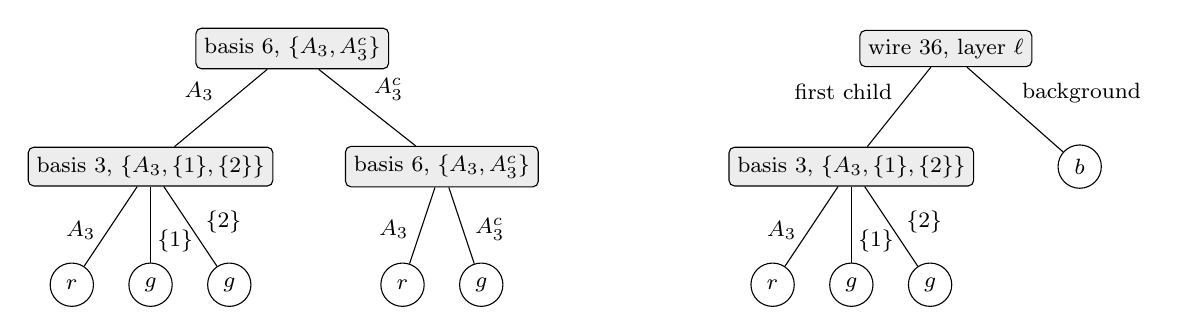
\begin{tikzpicture}[x=1cm,y=1cm,
   inner/.style={draw=black,fill=black!7,rounded corners=2pt,inner xsep=3pt,inner ysep=3pt,font=\footnotesize},
   leaf/.style={draw=black,circle,inner sep=1pt,minimum size=5.5mm,font=\footnotesize},
   every node/.style={font=\footnotesize}]
\begin{scope}
 \node[inner] (w) at (0,0) {basis $6$, $\{A_3,A_3^c\}$};
 \node[inner] (u) at (-1.8,-1.5) {basis $3$, $\{A_3,\{1\},\{2\}\}$};
 \node[inner] (v) at (1.9,-1.5) {basis $6$, $\{A_3,A_3^c\}$};
 \node[leaf] (u1) at (-2.8,-3.0) {$\col r$};
 \node[leaf] (u2) at (-1.8,-3.0) {$\col g$};
 \node[leaf] (u3) at (-0.8,-3.0) {$\col g$};
 \node[leaf] (v1) at (1.4,-3.0) {$\col r$};
 \node[leaf] (v2) at (2.4,-3.0) {$\col g$};
 \draw (w)-- node[above left=-1pt] {$A_3$} (u);
 \draw (w)-- node[above right=-1pt] {$A_3^c$} (v);
 \draw (u)-- node[left=1pt,pos=.55] {$A_3$} (u1);
 \draw (u)-- node[right=-1pt,pos=.72] {$\{1\}$} (u2);
 \draw (u)-- node[right=3pt,pos=.45] {$\{2\}$} (u3);
 \draw (v)-- node[left=1pt,pos=.55] {$A_3$} (v1);
 \draw (v)-- node[right=1pt,pos=.55] {$A_3^c$} (v2);
\end{scope}
\begin{scope}[xshift=8.3cm]
 \node[inner] (n) at (0,0) {wire $36$, layer $\ell$};
 \node[inner] (u) at (-1.2,-1.5) {basis $3$, $\{A_3,\{1\},\{2\}\}$};
 \node[leaf] (b) at (1.7,-1.5) {$\col b$};
 \node[leaf] (u1) at (-2.2,-3.0) {$\col r$};
 \node[leaf] (u2) at (-1.2,-3.0) {$\col g$};
 \node[leaf] (u3) at (-0.2,-3.0) {$\col g$};
 \draw (n)-- node[above left=-1pt] {first child} (u);
 \draw (n)-- node[above right=-1pt] {background} (b);
 \draw (u)-- node[left=1pt,pos=.55] {$A_3$} (u1);
 \draw (u)-- node[right=-1pt,pos=.72] {$\{1\}$} (u2);
 \draw (u)-- node[right=3pt,pos=.45] {$\{2\}$} (u3);
\end{scope}
\end{tikzpicture}
\caption{Two presentations at level $2$, with the colors $\col r,\col g,\col b$ of Section~\ref{sec:example} as scalars. Every edge is labeled by the part, or by the wire coordinate, to which the child belongs. Left: a presentation of the vertex $w=\bigl(6,(u,v,v,u)\bigr)$ of Section~\ref{sec:example}. The root is a basis node with the binary template at basis $6$, and its two children present $u=(3,\col{rggr})$ and $v=(6,\col{rggr})$. The tree has three internal nodes and no wire node. Right: a presentation of a vertex in layer $\ell$ of the wire along the edge $36$. The first child of the wire node presents $u$. The background of the wire node is the scalar $\col b$, which sits at level $1$ and is therefore padded to the constant word $\col{bbbb}$ in basis $6$. The tree has two internal nodes, one of which is a wire node.}
\label{fig:presentation}
\end{figure}

\begin{definition}\label{def:sparse-graph}
For $j,R\ge1$ and $\lambda=\max\{R-2,0\}$, let $G_{j,R}$ be the subgraph of $S^j_\lambda(K_3)$ induced by the vertices admitting a presentation with at most $2j-1$ internal nodes and at most $j$ wire nodes.
\end{definition}

We call $(G_{j,R})$ the \emph{sparse family}. Distinct presentations evaluating to the same vertex of $S^j_\lambda(K_3)$ produce a single vertex of $G_{j,R}$, and $G_{j,R}$ retains every edge of the full iterate between its vertices, including edges between vertices described by different trees. At level $j=1$, every vertex of $S_\lambda(K_3)$ has a presentation with a single internal node---a ternary basis node for a word of a basis chart, a wire node for a vertex of an interior layer---so $G_{1,R}=S_\lambda(K_3)$.

\subsection{The box complex and its first Stiefel--Whitney class}\label{sec:box}

To bound $\chi(S^j_\lambda(K_3))$ and $\chi(G_{j,R})$ from below at every level $j$, we use an equivariant topological invariant of graphs~\cite{Mat,Kozlov}. Every proper coloring sends the two sides of any complete bipartite subgraph to disjoint color sets; the box complex organizes all such bipartite pairs into a single topological space.

For a finite loopless graph $H$, the \emph{box complex} $\B(H)$ is the space of all ordered pairs $(\mu,\nu)$ of probability measures on $V(H)$ such that every vertex in $\operatorname{supp}\mu$ is adjacent in $H$ to every vertex in $\operatorname{supp}\nu$. It carries the subspace topology inherited from the product of two probability simplices. The two supports $\operatorname{supp}\mu$ and $\operatorname{supp}\nu$ are called the \emph{shores} of $(\mu,\nu)$.

Because $H$ is loopless, the two shores are disjoint, so swapping them, $(\mu,\nu)\mapsto(\nu,\mu)$, is a free continuous involution on $\B(H)$. A continuous map between spaces with involutions is \emph{equivariant} if it commutes with the involutions. Any graph homomorphism $f:G\to H$ induces an equivariant continuous map $\B(G)\to\B(H)$ by pushing both probability measures forward along $f$.

The space $\B(H)$ is the complex $\operatorname{Hom}(K_2,H)$ (surveyed in~\cite{Kozlov}), which is one of several models of the box complex. For connected graphs, Csorba~\cite[Theorem~9]{Csorba} shows that the barycentric subdivision of the simplicial box complex of Matou{\v s}ek and Ziegler~\cite{MZ} collapses equivariantly onto that of $\operatorname{Hom}(K_2,H)$. The two models are therefore equivariantly homotopy equivalent, so both admit the same equivariant maps to spheres and carry the same Stiefel--Whitney class defined below.

For the complete graph $K_p$ ($p\ge2$), two shores are completely adjacent precisely when they are disjoint. Consequently, the map $(\mu,\nu)\mapsto\mu-\nu$ identifies $\B(K_p)$ homeomorphically with the $\ell_1$-sphere of radius $2$ in the $(p-1)$-dimensional hyperplane $\{x\in\R^p:\sum_{a=1}^p x_a=0\}$, with inverse taking normalized positive and negative parts. Radial projection identifies this sphere equivariantly with the Euclidean $(p-2)$-sphere $S^{p-2}$ carrying the antipodal involution. Every proper $p$-coloring $H\to K_p$ therefore induces an equivariant continuous map $\B(H)\to S^{p-2}$. For $p=3$, the space $\B(K_3)$ is a hexagon---homeomorphic to the circle $S^1$ with shore exchange acting as the antipodal half-turn.

Any free involution $T$ on a compact polyhedron $Z$ defines a double cover $Z\to Z/\{1,T\}$ and hence a cohomology class $w_Z\in H^1(Z/\{1,T\};\Ftwo)$, the \emph{first Stiefel--Whitney class} of the double cover~\cite{MS}. Evaluated on a closed loop in $Z/\{1,T\}$, the class $w_Z$ equals $1$ if a lift of the loop to $Z$ switches sheets and $0$ if it closes up. An equivariant map $Z\to Y$ pulls back $w_Y$ to $w_Z$. In particular, if $Z$ admits an equivariant map to $\B(H)$ and $w_Z^k\ne0$ in $H^k(Z/\{1,T\};\Ftwo)$, then
\begin{equation}\label{eq:classical-obstruction}
 \chi(H)\ge k+2.
\end{equation}
Indeed, composing $Z\to\B(H)$ with the equivariant map $\B(H)\to S^{p-2}$ from a $p$-coloring descends to a map $Z/\{1,T\}\to\mathbb{RP}^{p-2}$ pulling back the generator of $H^1(\mathbb{RP}^{p-2};\Ftwo)$ to $w_Z$. Since $H^k(\mathbb{RP}^{p-2};\Ftwo)=0$ for $k>p-2$, $w_Z^k\ne0$ forces $p-2\ge k$, i.e., $p\ge k+2$. For $Z=\B(H)$, we write simply $w=w_{\B(H)}$ and call the largest integer $k$ with $w^k\ne0$ the \emph{height} of $w$.

\subsection{Towers and the substitution step}\label{sec:towers}

To lift the obstruction~\eqref{eq:classical-obstruction} inductively across each substitution, we mirror the graph operation $S_\lambda$ on topological spaces carrying a free circle action.

A \emph{circle space} is a compact polyhedron $X$ equipped with a free continuous action of the circle group $S^1=\{z\in\C:|z|=1\}$. Its \emph{half-turn} is the action $T(x)=(-1)\cdot x$, which is a free involution on $X$. Given a circle space $X$, the space $S(X)$ is defined in the same way as the graph $S_\lambda(H)$.
\begin{itemize}
\item \emph{Basis blocks.} A \emph{basis block} is the subspace of tuples $(x_0,x_1,x_2,x_3)\in X^4$ that satisfy $x_0=x_r$ for some $r\in\{1,2,3\}$. Take six disjoint basis blocks, one for each basis $i\in\{1,\ldots,6\}$.
\item \emph{Cylinders.} For each edge $e=ik$ of $K_{3,3}$ (with $i\le3<k$), take a cylinder $X^2\times[0,1]$.
\item \emph{Attachments.} For each edge $e=ik$, identify the point $(x,y,0)$ of its cylinder with the tuple in basis block $i$ that takes $x$ on $A_{i,e}$ and $y$ on $A_{i,e}^c$, and identify the point $(x,y,1)$ with the tuple in basis block $k$ that takes $x$ on $A_{k,e}$ and $y$ on $A_{k,e}^c$. These are the coordinate repetitions of $S_\lambda$.
\end{itemize}
Rotating all coordinates simultaneously defines a free continuous $S^1$-action, which makes $S(X)$ a circle space (verified in Appendix~\ref{app:cont-pres}).

Work with normalized singular chains over $\Ftwo$. For a chain $c$ in a circle space, let $Bc$ denote the chain swept out by $c$ during one full rotation of $S^1$ (defined precisely via the shuffle chain action before~\eqref{eq:circle-chain} in Appendix~\ref{app:cont-pres}). A \emph{tower of length $h$} on a circle space $Z$ consists of a $0$-chain $x_0$ given by a single point together with chains $x_1,\ldots,x_h$, where $x_i$ has dimension $2i$, satisfying
\begin{equation}\label{eq:tower}
 \partial x_i=Bx_{i-1}\qquad (1\le i\le h).
\end{equation}
Thus a tower of length $0$ is simply a point, and a tower of length $1$ is a point together with a $2$-chain whose boundary is the $S^1$-orbit of that point. A \emph{tower of length $h$ over a graph $G$} consists of a circle space $Z$ with a tower of length $h$ together with a continuous map $Z\to\B(G)$ that is equivariant for the half-turn $T$ on $Z$ and shore exchange on $\B(G)$. We say that a circle space (or graph) \emph{carries} a tower of length $h$ if such a tower exists on it (respectively, over it).

A tower of length $h$ forces $2h+1$ nonvanishing powers of the Stiefel--Whitney class.

\begin{proposition}[Towers bound the chromatic number]\label{prop:tower-bound}
If there is a tower of length $h$ over $G$, then $w^{2h+1}\ne0$ on $\B(G)$ and $\chi(G)\ge2h+3$.
\end{proposition}
\begin{proof}
Let $Z\to\B(G)$ be the equivariant map of a tower of length $h$ over $G$. Lemma~\ref{lem:tower-detection} in Appendix~\ref{app:tower-det} shows that $w_Z^{2h+1}\ne0$. Because $w_Z$ is the pullback of $w$ along $Z\to\B(G)$, we also have $w^{2h+1}\ne0$ on $\B(G)$. Applying~\eqref{eq:classical-obstruction} with $k=2h+1$ yields $\chi(G)\ge2h+3$.
\end{proof}

The heart of our classical lower bound is that each square substitution extends any tower by one step.

\begin{theorem}[Substitution step]\label{thm:step}
If there is a tower of length $h$ over a graph $H$, on a circle space $X$, then for every $\lambda\ge0$ there is a tower of length $h+1$ over $S_\lambda(H)$, on the circle space $S(X)$. Consequently, for every $j\ge0$,
\[
 w^{2(h+j)+1}\ne0\ \text{ on }\B(S^j_\lambda(H)),\qquad \chi(S^j_\lambda(H))\ge2(h+j)+3.
\]
\end{theorem}
\begin{proof}
Let $x_0,\ldots,x_h$ be a tower of length $h$ on $X$ with equivariant map $X\to\B(H)$. Appendix~\ref{app:cont-pres} shows that $S(X)$ is a circle space. Lemma~\ref{lem:square-tower}(a) in Appendix~\ref{app:cont-pres} produces a tower of length $h+1$ on $S(X)$, and Lemma~\ref{lem:box-realization} in Appendix~\ref{app:box-real} lifts $X\to\B(H)$ to an equivariant map $S(X)\to\B(S_\lambda(H))$. Together these form a tower of length $h+1$ over $S_\lambda(H)$. Applying this step $j$ times produces a tower of length $h+j$ over $S^j_\lambda(H)$, and Proposition~\ref{prop:tower-bound} yields both displayed conclusions.
\end{proof}

Before turning to the applications, we explain the cancellation behind Lemma~\ref{lem:square-tower}. Consider first a tower of length $0$, which is a single point $x_0$ of $X$. A tower of length $1$ on $S(X)$ consists of a point of $S(X)$ and a $2$-chain whose boundary is the $S^1$-orbit of that point. The point will be the constant tuple $(x_0,x_0,x_0,x_0)$ in basis block $6$, and we have to show that its orbit is a boundary over $\Ftwo$.

Let $b$ be a basis, and let $D$ be either a part of a template at $b$ or the set $\{0,1,2,3\}$ of all positions. Let $\gamma_{b,D}$ be the loop in basis block $b$ along which the entries at the positions in $D$ run once around the orbit of $x_0$, while the other entries stay at $x_0$. For $D=\{0,1,2,3\}$ this loop is the orbit of the constant tuple of block $b$, and we denote it by $o_b$. In homology with coefficients in $\Ftwo$, the loops satisfy two kinds of relations.
\begin{itemize}
\item \emph{Templates.} A template at $b$ with parts $D_1,\ldots,D_p$ defines a map from $X^p$ into block $b$, which repeats its $m$th argument at the positions of $D_m$. This map sends the product of $p$ copies of the orbit of $x_0$ onto a torus. On a torus, the diagonal loop is homologous to the sum of the coordinate loops. Hence $o_b$ is homologous to $\gamma_{b,D_1}+\cdots+\gamma_{b,D_p}$.
\item \emph{Wires.} The cylinder of an edge $e=ik$ carries the loop $\gamma_{i,A_{i,e}}$ to the loop $\gamma_{k,A_{k,e}}$, and the orbit $o_i$ to the orbit $o_k$. Hence $\gamma_{i,A_{i,e}}$ is homologous to $\gamma_{k,A_{k,e}}$, and all six orbits $o_b$ are homologous to one another.
\end{itemize}
Now add the relations of all nineteen templates. On the left there are nineteen orbits. On the right, the loops occur as follows.
\[
\begin{array}{c|c|c}
\text{Basis }b & \text{Loops that occur twice} & \text{Loops that occur once}\\ \hline
1,\ldots,5 & \gamma_{b,\{1\}},\ \gamma_{b,\{2\}},\ \gamma_{b,\{3\}} & \gamma_{b,A_1},\ \gamma_{b,A_2},\ \gamma_{b,A_3}\\
6 & \gamma_{6,\{1\}},\ \gamma_{6,\{2\}},\ \gamma_{6,\{3\}},\ \gamma_{6,A_3} & \gamma_{6,A_1},\ \gamma_{6,A_2},\ \gamma_{6,A_3^c}
\end{array}
\]
At every basis, each singleton belongs to two of the three ternary templates and each set $A_r$ to one of them. At basis $6$, the binary template $\{A_3,A_3^c\}$ contributes $\gamma_{6,A_3}$ a second time and adds $\gamma_{6,A_3^c}$. Loops that occur twice cancel modulo $2$. By Table~\ref{tab:edges}, the eighteen loops that occur once are exactly the loops $\gamma_{b,A_{b,e}}$ at the two ends of the nine edges $e$ of $K_{3,3}$, so they cancel in pairs along the wires. The right-hand side therefore vanishes in homology. Since nineteen is odd and the orbits $o_b$ are homologous to one another, the left-hand side is homologous to $o_6$. Thus $o_6$ is a boundary, as required. Without the binary template the count would prove nothing: the loops $\gamma_{3,A_3}$ and $\gamma_{6,A_3}$ would remain unpaired, and the number of orbits would be even.

For a tower $x_0,\ldots,x_h$ of arbitrary length, Lemma~\ref{lem:square-tower} carries out the same count with chains in place of loops. For each of the nineteen templates it forms a product of the chains of the tower over the parts of the template. The boundary terms that do not cancel within one template are \emph{insertions}: the chain $Bx_h$, swept out by the last chain of the tower, placed on a single part $D$ at a basis $b$, with the base point $x_0$ at all other positions. Insertions cancel as the loops $\gamma_{b,D}$ do in the array above. Those that occur twice cancel modulo $2$, and the remaining eighteen are the two ends of the nine cylinders $X^2\times[0,1]$, along which the inserted chain is swept. In dimension $0$, the constant tuple on $x_0$ occurs $3+3$ times in each of the blocks $1,\ldots,5$, from three templates and three wire ends, and $4+3$ times in block $6$. Over $\Ftwo$ only the constant tuple in block $6$ remains, and it is the base point of the new tower.

\subsection{The chromatic gap and sparse size bounds}\label{sec:gap-results}

All pieces are now in place to prove the chromatic gap for the full iterates $S^j_\lambda(K_3)$ and for the sparse family $G_{j,R}$.

\begin{theorem}[The gap]\label{thm:gap}
For all $j\ge1$ and $\lambda\ge0$, the graph $S^j_\lambda(K_3)$ has quantum chromatic number three and classical chromatic number at least $2j+3$. The strategy above is a $(\lambda+2)$-compatible quantum $3$-coloring in local dimension $4^j$.
\end{theorem}
\begin{proof}
\emph{Quantum $3$-coloring.} The scalar projectors on $K_3$ commute at every distance. Applying Lemma~\ref{lem:radius-lift} inductively $j$ times with $R=\lambda+2$ shows that the $j$-fold iterate of~\eqref{eq:strategy} is a $(\lambda+2)$-compatible quantum $3$-coloring of $S^j_\lambda(K_3)$ in local dimension $4^j$. Moreover, starting from $K_3$, the constant words in any basis chart on the vertices of a triangle again form a triangle; by induction, $S^j_\lambda(K_3)$ contains a triangle, so $\cq(S^j_\lambda(K_3))=3$.

\emph{Classical lower bound.} As shown in Section~\ref{sec:box}, $\B(K_3)$ is a circle on which shore exchange acts as the half-turn. Taking $X=\B(K_3)$ with the identity map and any single point $x_0\in\B(K_3)$ gives a tower of length $h=0$ over $K_3$. Theorem~\ref{thm:step} applied with $h=0$ yields $\chi(S^j_\lambda(K_3))\ge2j+3$.
\end{proof}

Section~\ref{sec:rigidity} proves that neither the local dimension $4^j$ nor the compatibility radius $\lambda+2$ can be improved on $S^j_\lambda(K_3)$.

\begin{remark}\label{rem:tables}
For $\lambda=0$, every vertex of $S^j_0(K_3)$ is a basis word at every level. Its measurement in the $j$-fold iterate of~\eqref{eq:strategy} is therefore that of a \emph{table}. A table chooses one of the six bases for every sequence of fewer than $j$ positions, the empty sequence included; this is the basis in which the next two-qubit register is measured. It also chooses one of the three colors for every sequence of $j$ positions. Let $M_j$ be the physical graph on the measurements of all $6^{(4^j-1)/3}3^{4^j}$ tables. Adjacent vertices of $S^j_0(K_3)$ carry measurements that are orthogonal at every color, hence distinct and adjacent in $M_j$, so $\chi(M_j)\ge\chi(S^j_0(K_3))\ge2j+3$ by Theorem~\ref{thm:gap}. Moreover, $\cq(M_j)=3$, because the measurements themselves form a quantum $3$-coloring of $M_j$ in local dimension $4^j$ and the three constant measurements form a triangle.
\end{remark}

The order of $S^j_\lambda(K_3)$ grows doubly exponentially in $j$, because one substitution turns an $n$-vertex graph into a graph on $6(n^4-n(n-1)^3)+9\lambda n^2$ vertices. Restricting to bounded presentations reduces the order and edge count to singly exponential in $j$ while preserving every property of Theorem~\ref{thm:gap}.

\begin{theorem}[The sparse family]\label{thm:sparse}
There is an absolute constant $C$ such that, for all $j,R\ge1$, the graph $G_{j,R}$ satisfies
\[
 \cq(G_{j,R})=3,\qquad \chi(G_{j,R})\ge2j+3,\qquad |V(G_{j,R})|+|E(G_{j,R})|\le[C(1+R)]^j.
\]
The strategy of Theorem~\ref{thm:gap} restricts to an $R$-compatible quantum $3$-coloring of $G_{j,R}$ in local dimension $4^j$, and $w^{2j+1}\ne0$ on $\B(G_{j,R})$. The graph and the projectors in~\eqref{eq:strategy} can be generated deterministically in $\exp(O(j\log(R+2)))$ bit operations, with an absolute implicit constant.
\end{theorem}
\begin{proof}
We establish in turn the quantum coloring, the topological classical lower bound, the vertex and edge counts, and the deterministic generation bound. Throughout, set $\lambda=\max\{R-2,0\}$.

\emph{Quantum $3$-coloring.} Because $G_{j,R}$ is a subgraph of $S^j_\lambda(K_3)$, every path in $G_{j,R}$ is also a path in $S^j_\lambda(K_3)$, so $\dist_{S^j_\lambda(K_3)}(u,v)\le\dist_{G_{j,R}}(u,v)$. Restricting the $(\lambda+2)$-compatible strategy of Theorem~\ref{thm:gap} to $G_{j,R}$ therefore gives a $(\lambda+2)$-compatible, hence $R$-compatible, quantum $3$-coloring in local dimension $4^j$. The three padded scalar leaves $0,1,2$ form a triangle in $G_{j,R}$, so $\cq(G_{j,R})=3$.

\emph{Classical lower bound.} Start from the circle $X_0=S^1=\B(K_3)$ and form the iterated circle spaces $X_{h+1}=S(X_h)$. Padding the starting circle diagonally in basis block $6$ produces a distinguished orbit $O_h\subset X_h$ at every level $h$. As detailed in Appendix~\ref{app:cont-pres}, let $Z_{j,j}\subset X_j$ be the compact polyhedron of points admitting a continuous presentation with at most $2j-1$ internal nodes and at most $j$ wire nodes, using points of $O_h$ at scalar leaves and parameters in $[0,1]$ on wires. By Appendix~\ref{app:cont-pres}, $Z_{j,j}$ is a circle space. Lemma~\ref{lem:square-tower}(b) constructs a tower $x_0,\ldots,x_j$ on $X_j$ with each $x_i$ supported in $Z_{j,i}\subseteq Z_{j,j}$, hence a tower of length $j$ on $Z_{j,j}$. By Lemma~\ref{lem:box-realization} in Appendix~\ref{app:box-real}, the $j$-fold iterated map $X_j\to\B(S^j_\lambda(K_3))$ sends $Z_{j,j}$ equivariantly into $\B(G_{j,R})$. Thus $G_{j,R}$ carries a tower of length $j$, and Proposition~\ref{prop:tower-bound} gives both $w^{2j+1}\ne0$ on $\B(G_{j,R})$ and $\chi(G_{j,R})\ge2j+3$.

\emph{Vertex count.} Temporarily erase all interior layer indices $\ell\in\{1,\ldots,\lambda\}$ from a presentation meeting Definition~\ref{def:sparse-graph}, keeping at each wire node its edge $e$ of $K_{3,3}$ and a three-way tag indicating layer $0$, layer $\lambda+1$, or an interior layer. An ordered tree with at most $2j-1$ internal nodes of arity at most $3$ has at most $6j-2=O(j)$ nodes in total. Recording its preorder traversal of node arities and labels from a fixed finite alphabet shows that at most $C_0^j$ such stripped trees exist for an absolute constant $C_0$. Restoring the interior layer index at each of the at most $j$ wire nodes multiplies this count by at most $(1+\lambda)^j$. Since every vertex of $G_{j,R}$ has at least one valid presentation, $|V(G_{j,R})|\le C_0^j(1+\lambda)^j$.

\emph{Edge count.} We bound pairs of presentations whose evaluated vertices are adjacent in $S^j_\lambda(K_3)$. If $\lambda\le1$, then $|V(G_{j,R})|\le (2C_0)^j$, so $|E(G_{j,R})|\le (2C_0)^{2j}$, which already has the desired form after increasing the constant. Assume now that $\lambda\ge2$. Fix a pair of stripped trees $(\Gamma_1,\Gamma_2)$ (at most $C_0^{2j}$ pairs) and fix a complete assignment of interior layer numbers to $\Gamma_2$ (at most $(1+\lambda)^j$ choices). We bound the number of interior layer assignments to $\Gamma_1$ that produce an edge between the evaluated vertices of $\Gamma_1$ and $\Gamma_2$.

Expand every wire node labeled as an endpoint ($\ell=0$ or $\ell=\lambda+1$) in $\Gamma_1$ and $\Gamma_2$ into its equivalent basis word, and read padded scalar leaves at whatever level is required; neither expansion introduces any new interior layer variable. Now test adjacency recursively from the root down to level $0$. At any current pair of nodes $(u_1,u_2)$ at the same level:
\begin{enumerate}
\item If both $u_1$ and $u_2$ are basis words, adjacency forces them to lie in the same basis and their four child entries to be coordinatewise adjacent.
\item If both $u_1$ and $u_2$ are interior wire nodes, adjacency forces them to lie on the same wire $e$, their layer indices $\ell_1,\ell_2$ to satisfy $|\ell_1-\ell_2|\le1$ (leaving at most $3$ choices for $\ell_1$ given $\ell_2$), and their two pairs of children to be coordinatewise adjacent.
\item If exactly one of $u_1,u_2$ is an interior wire node and the other is a basis word, adjacency forces the basis word to lie at one endpoint of that wire and forces the interior layer index to equal $1$ (if adjacent to layer $0$) or $\lambda$ (if adjacent to layer $\lambda+1$). In particular, if $u_1$ is the interior node, $\ell_1$ is uniquely determined, and adjacency requires coordinatewise adjacency across all four positions, reading the two children of the interior wire node on $A_{b,e}$ and $A_{b,e}^c$.
\end{enumerate}
These necessary adjacency comparisons recursively visit every interior wire node of $\Gamma_1$ (if a child subtree occurs at several positions of a parent word, keep the constraint from the first comparison that visits it). Each interior wire node of $\Gamma_1$ thus has either $1$ or at most $3$ compatible layer indices once $\Gamma_2$'s layers are fixed. With at most $j$ wire nodes in $\Gamma_1$, at most $3^j$ assignments on $\Gamma_1$ can produce an edge to $\Gamma_2$. Summing over all $(\Gamma_1,\Gamma_2)$ and all layer assignments on $\Gamma_2$ gives at most $C_0^{2j}(1+\lambda)^j 3^j$ adjacent pairs; multiple presentations of the same vertex only overcount. Because $1+\lambda\le 1+R$, we conclude $|V(G_{j,R})|+|E(G_{j,R})|\le[C(1+R)]^j$ for an absolute constant $C$.

\emph{Deterministic generation.} To build $G_{j,R}$, enumerate all bounded presentation trees, expand each recursively to a canonical vertex label in $S^j_\lambda(K_3)$, sort to remove duplicates, and run the defining adjacency test of $S^j_\lambda(K_3)$ on every pair (including, when $\lambda=0$, cross-basis endpoint pairs on a common wire). Expanding a label and testing a pair each require at most $C_1^j$ elementary operations on symbols and layer indices of $O(\log(R+2))$ bits. Even checking all pairs of presentations takes at most $[C_2(1+R)]^{2j}C_1^j\cdot O(\log(R+2))=\exp(O(j\log(R+2)))$ bit operations. Finally, every matrix $Q^i_s$ and $P_e$ has entries in $\tfrac14\mathbb Z$, so the iterated $4^j\times 4^j$ projectors in~\eqref{eq:strategy} have rational entries of magnitude at most $1$ with common denominator $4^j$; computing them recursively from~\eqref{eq:strategy} fits within the same bit-operation bound.
\end{proof}

The lower bound of Theorem~\ref{thm:sparse} is sharp up to a constant factor when $R\ge3$, and nearly so when $R\le2$.

\begin{corollary}[Linear growth on the sparse family]\label{cor:linear-growth}
There is an absolute constant $K$ such that, for all $j\ge1$ and $R\ge3$,
\[
 2j+3\le\chi(G_{j,R})\le Kj .
\]
For $R\in\{1,2\}$, the graphs $G_{j,1}=G_{j,2}$ satisfy $\chi(G_{j,1})=O(j^{1+\beta})$ with $\beta=\log_2(18/17)<0.083$. Consequently, every quantum $3$-coloring of $G_{j,R}$ has local dimension at least $4^{\chi(G_{j,R})/K}$ if $R\ge3$, and at least $\exp\bigl(\Omega(\chi(G_{j,R})^{1/(1+\beta)})\bigr)$ if $R\le2$.
\end{corollary}
\begin{proof}
The lower bound is Theorem~\ref{thm:sparse}. Let $R\ge3$, so that $\lambda=R-2\ge1$, and put $t=\chi(G_{j,R})$. Every vertex of $G_{j,R}$ admits a presentation, so Proposition~\ref{prop:readings} in Appendix~\ref{app:readings} and the order bound of Theorem~\ref{thm:sparse} give
\[
 \Bigl(\frac{9R-17}{2}\Bigr)^{\lfloor(t-1)/3\rfloor}\le|V(G_{j,R})|\le[C(1+R)]^j,
\]
where we may assume $C\ge1$. Since $(9R-17)/2\ge1+R\ge4$ for $R\ge3$, taking logarithms gives $\lfloor(t-1)/3\rfloor\le j\,(1+\log C/\log4)$, and $t\le3\lfloor(t-1)/3\rfloor+3$. This proves the upper bound with $K=6+3\log C/\log4$. The bound for $R\le2$ is Proposition~\ref{prop:zero-layer}. For the last assertion, Theorem~\ref{thm:dimension} below shows that every quantum $3$-coloring of $G_{j,R}$ has local dimension at least $4^j$, and the two upper bounds give $j\ge\chi(G_{j,R})/K$ and $j=\Omega(\chi(G_{j,R})^{1/(1+\beta)})$, respectively.
\end{proof}

The proof colors $G_{j,R}$ by composing random maps from each level to the preceding one. Such a map can respect all nine wires only if one of them is cut, and the scalar backgrounds of the presentations keep the loss at each cut bounded. Neither feature is available for the full iterates, whose growth remains open (Problem~\ref{prob:growth}).
